\documentclass[conference]{IEEEtran}
\IEEEoverridecommandlockouts
% The preceding line is only needed to identify funding in the first footnote. If that is unneeded, please comment it out.
\usepackage{cite}
\usepackage{amsmath,amssymb,amsfonts}
\usepackage{algorithmic}
\usepackage{textcomp}
\usepackage{theorem,caption,extarrows,mathrsfs,physics,bm}
\usepackage{graphicx,xcolor,booktabs,subfigure,tikz}
\usepackage{pgfplots,grffile}
\usepackage{fontspec,xeCJK}
\setmainfont{TeX Gyre Termes}
\usepackage[skins]{tcolorbox}
\usepackage{listings}
\lstset{
    basicstyle          =   \sffamily,          % 基本代码风格
    keywordstyle        =   \bfseries,          % 关键字风格
    commentstyle        =   \rmfamily\itshape,  % 注释的风格,斜体
    stringstyle         =   \ttfamily,  % 字符串风格
    flexiblecolumns,                % 别问为什么,加上这个
    numbers             =   left,   % 行号的位置在左边
    showspaces          =   false,  % 是否显示空格,显示了有点乱,所以不现实了
    numberstyle         =   \tiny\ttfamily,    % 行号的样式,小五号,tt等宽字体
    showstringspaces    =   false,
    captionpos          =   t,      % 这段代码的名字所呈现的位置,t指的是top上面
    frame               =   shadowbox,   % 显示边框
    rulesepcolor=\color{red!20!green!20!blue!20}
}

\lstdefinestyle{Python}{
    language        =   Python, % 语言选Python
    backgroundcolor=\color{backpycol},
    basicstyle      =   \ttfamily,
    numberstyle     =   \ttfamily,
    keywordstyle    =   \color{blue},
    keywordstyle    =   [2] \color{teal},
    stringstyle     =   \color{magenta},
    commentstyle    =   \color[HTML]{338AAF}\ttfamily,
    breaklines      =   true,   % 自动换行,建议不要写太长的行
    columns         =   fixed,  % 如果不加这一句,字间距就不固定,很丑,必须加
    basewidth       =   0.5em,
}
\definecolor{codegreen}{rgb}{0,0.6,0}
\definecolor{codegray}{rgb}{0.5,0.5,0.5}
\definecolor{codepurple}{rgb}{0.58,0,0.82}
\definecolor{backcolour}{rgb}{0.95,0.95,0.92}
\definecolor{backpycol}{rgb}{0.97,0.95,0.97}
\lstdefinestyle{C++}{
    language =[ANSI]C,
    backgroundcolor=\color{backcolour},
    commentstyle=\color[HTML]{338AAF}\ttfamily,
    keywordstyle=\sffamily\bfseries\color{magenta},
    numberstyle=\color{codegray},
    stringstyle=\color{codepurple},
    basicstyle=\ttfamily,
    breakatwhitespace=false,
    breaklines=true,
    basewidth=0.5em,
    captionpos=b,
    columns=fixed,
    frame=shadowbox,
    keepspaces=true,
    numbers=left,
    numbersep=5pt,
    showspaces=false,
    showstringspaces=false,
    showtabs=false,
    tabsize=4
}
\lstdefinestyle{matlab}{
    language=matlab,
    backgroundcolor=\color{backcolour},
    commentstyle=\color[HTML]{338AAF}\ttfamily,
    keywordstyle=\sffamily\bfseries\color{magenta},
    numberstyle=\color{codegray},
    stringstyle=\color{codepurple},
    basicstyle=\ttfamily,
    breakatwhitespace=false,
    breaklines=true,
    basewidth=0.5em,
    captionpos=b,
    columns=fixed,
    keepspaces=true,
    numbers=left,
    numbersep=5pt,
    showspaces=false,
    showstringspaces=false,
    showtabs=false,
    tabsize=4,
    frame=shadowbox
}
\definecolor{mygreen}{rgb}{0,0.6,0}
\definecolor{mygray}{rgb}{0.5,0.5,0.5}
\definecolor{mymauve}{rgb}{0.58,0,0.82}
\definecolor{bggray}{rgb}{0.93,0.95,0.94}
\lstdefinestyle{pseudocode}{
    backgroundcolor=\color{bggray},
    columns=fullflexible,
    tabsize=4,
    breaklines=true,               % automatic line breaking only at whitespace
    captionpos=b,                  % sets the caption-position to bottom
    commentstyle=\color{mygreen},  % comment style
    escapeinside={\%*}{*)},        % if you want to add LaTeX within your code
    keywordstyle=\color{blue},     % keyword style
    stringstyle=\color{mymauve}\ttfamily,  % string literal style
    frame=shadowbox,
    rulesepcolor=\color{red!20!green!20!blue!20},
    % identifierstyle=\color{red},
    language=c++,
    numbers=left,
    numberstyle=\small\color{codegray},
    basicstyle=\ttfamily,% size of fonts used for the code
    escapeinside=``,
    xleftmargin=0.6em,
    xrightmargin=0.6em,
    aboveskip=1em
}
\lstdefinestyle{Fortran}{
    language =fortran,
    backgroundcolor=\color{backcolour},
    commentstyle=\color[HTML]{338AAF}\ttfamily,
    keywordstyle=\sffamily\bfseries\color{magenta},
    numberstyle=\small\color{codegray},
    stringstyle=\color{codepurple},
    basicstyle=\ttfamily,
    breakatwhitespace=false,
    breaklines=true,
    basewidth=0.5em,
    captionpos=b,
    columns=fixed,
    frame=shadowbox,
    keepspaces=true,
    numbers=left,
    numbersep=5pt,
    showspaces=false,
    showstringspaces=false,
    showtabs=false,
    tabsize=4
}
\setmonofont{CMU Typewriter Text}
\pgfplotsset{compat=newest}
  %% the following commands are needed for some matlab2tikz features
\usetikzlibrary{plotmarks}
\usetikzlibrary{arrows.meta}
\usetikzlibrary{calc}
\usepgfplotslibrary{patchplots}
\def\BibTeX{{\rm B\kern-.05em{\sc i\kern-.025em b}\kern-.08em
    T\kern-.1667em\lower.7ex\hbox{E}\kern-.125emX}}
%% Define the theorem and proof
\newtheorem{theorem}[subsection]{Theorem}
\newtheorem{definition}[subsection]{Definition}
\newenvironment{thmbox}{\par
	\vspace{4pt}
	\begin{center}
	\tcbset{enhanced,notitle,colframe=black,colback=white}
	\begin{tcolorbox}[fuzzy shadow={1.6mm}{-1.6mm}{0mm}{0mm}{fill=black!90!white},arc=0mm]}{\end{tcolorbox}
	\end{center}}

\begin{document}
\title{Lab 5 Report: Fast Fourier Transform With MATLAB}

\author{IEEEauthorblockN{1\textsubscript{st} Qiu Kunyuan}
	\IEEEauthorblockA{\textit{EEE. Southern University of Science and Technology}\\
		Shenzhen, PRC\\
		11913019@mail.sustech.edu.cn}
}
\maketitle

\begin{abstract}
	This lab session conducts further discussions on the efficiency and computational cost of the discrete Fourier transformation(DFT). The matrix multiplication approach of the DFT is not only computationally intensive, but also consumes a lot of time for memory read and write operations when creating matrices. The theoretical complexity of DFT is \( \mathcal{O} (n^{2}) \), and the memory allocations involved in actual execution increases the time complexity of DFT further. In order to cut down the time complexity of DFT operations, which is intensively adopted in modern digital signal processing(DSP), a new algorithm using divide-conquer strategy is implemented and the theoretical complexity of DFT is reduced to \( \mathcal{O} (n\log_{2}n) \). This algorithm is named Fast Fourier Transformation(FFT) and is used widely today.
\end{abstract}

\begin{IEEEkeywords}
	FFT, time complexity, high-performance computation, MATLAB
\end{IEEEkeywords}

\section{Introduction}

\subsection{Frequency Range Shift}
The FFT result is a sequence with subscript \( k \) and the corresponding frequency range of the result is \( [0,2\pi ] \) rather than \( [-\pi ,\pi ] \). For a bandpass signal with bandwidth \( B \), its FFT result are not intuitive since the nonzero values locates in the interval \( [0,B] \cup [B,2\pi ]\). This property of the \textit{raw} FFT output make it difficult to process further.

To overcome this difficulty, a shift should be done so that the misplaced sequence is recovered. Let the desired shift be a map \( fftshift:X[k]\mapsto X[k] \), this map is defined as
\begin{equation}
	X[k-2\pi]=X[k],k\in[\pi,2\pi ]
\end{equation}

\subsection{Zero Padding}
The FFT requires the length of input sequence to be a integer power of 2. For a sequence with arbitrary length \( L \), the input sequence are padded with zero so that the length requirement is satisfied:
\begin{equation}
	N_{Z}=2^{\left\lceil \log_{2}L \right\rceil },x_{in}=[x,\text{zeros}(1,N_{Z}-L)]
\end{equation}

This technique can also be used to produce a finer sampling of the DTFT, for the frequency step is inversely proportional to the number of sampling points and the time domain multiplication with a step function equals to a frequency domain convolution with a sinc function.

\subsection{FFT Algorithm}
To boost the evaluation of the DFT, the divide-conquer strategy is tried since there are lots of preceding examples, such as Strassen method for matrix multiplication. The proportion of division is selected to 2, because multiplication or division of factor 2 is done by shift registers in digital circuit and the cost of each operation is one single clock pulse.

The DFT summation can be break into 2 parts, one is of odd indexes and the other is of even indexes:
\begin{equation}
	\begin{aligned}
		\mathcal{F} (x[t]) & =\sum_{t=0}^{N-1} x[t]\exp(-j \frac{2\pi t}{N}k)             \\
		                   & =\sum_{m=0}^{\frac{N}{2}-1} x[2m]\exp(-j \frac{2\pi 2m}{N}k) \\&+\sum_{m=0}^{\frac{N}{2}-1} x[2m+1]\exp(-j \frac{2\pi (2m+1)}{N}k)
	\end{aligned}
\end{equation}
The equation above can be rearranged into a prettier form:
\begin{equation}
	\begin{aligned}
		\mathcal{F} (x[n]) & =\sum_{m=0}^{\frac{N}{2}-1} x[2m]\exp(-j \frac{2\pi m}{N/2}k) \\&+\exp(-j \frac{2\pi}{N}k)\sum_{m=0}^{\frac{N}{2}-1} x[2m+1]\exp(-j \frac{2\pi m}{N/2}k)\\
		                   & =\mathcal{F}(x[2n])+\mathcal{F} (x[2n+1])W_{N}^{k}
	\end{aligned}
\end{equation}

With the deductions above, a recursion relation is established and the size of each recursion is half to the upper recursion step. The twiddle factor
\begin{equation}
	W_{N}^{k}=\exp(-j \frac{2\pi k}{N})
\end{equation}
is a vector in equation (5) for
\begin{lstlisting}
    k=0:length(x(l*n))
\end{lstlisting}
is a vector of length \( N/l \). Since the complex exponential factor, or the twiddle factor has the property that
\begin{equation}
	\exp \left( -j \frac{2\pi k+N/2}{N} \right) =-\exp \left( -j\frac{2\pi k}{N} \right)
\end{equation}
The recursion relation (4) can be simplified as
\begin{equation}
	\begin{matrix}
		X[k]=X_{0}[k]+W_{k}^{N}X_{1}[k] \\
		X[k+N/2]=X_{0}[k]-W_{N}^{k}X_{1}[k]
	\end{matrix},
	k\in[0,N/2-1]
\end{equation}

\subsection{Complexity Analysis}
Since the size of each sub-problem is halved after every single iteration, and the time consumption of the merging operation is \( \mathcal{O} (n) \), the time complexity can be then obtained by solving the recursion below:
\begin{equation}
	T(n)=2T(n/2)+O(n)\Rightarrow T(n)=O(n\log n)
\end{equation}

The fig.\ref{fig:theo_fft.png} visualizes the vast complexity gap between FFT and DFT explicitly.

\begin{figure}[htpb]
	\centering
	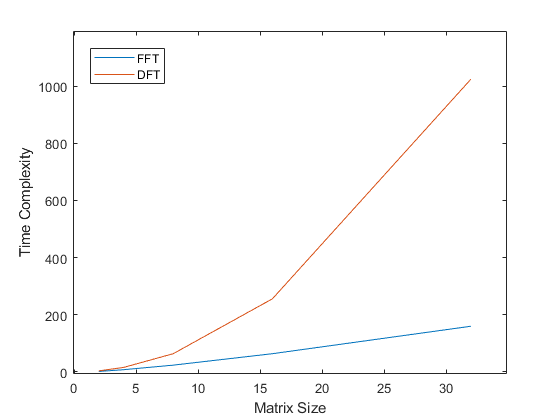
\includegraphics[width=0.45\textwidth]{theo_fft.png}
	\caption{Theoretical Time Complexity Plot}
	\label{fig:theo_fft.png}
\end{figure}

The recursion implementation of the FFT algorithm requires large stack memory due to the tail recursion. The avoidance of this problem leads to the conversion from tail recursion to nested loop, and sequential structure in terms of loop implementation is naturally suitable for MATLAB and FPGA programming.

\section{Frequency Range Shifting and Zero Padding}
\subsection{Frequency Range Shift}
The built-in function \lstinline{fftshift()} is applied to recover the \textit{misplaced} output sequence of original DFT function:

\lstinputlisting[language=matlab,style=matlab]{DTFTsamples.m}

Fig.\ref{fig:p521.png} clearly demonstrates that the shifting recovers the order of output sequence comparing to the original DFT output.

\begin{figure}[htpb]
	\centering
	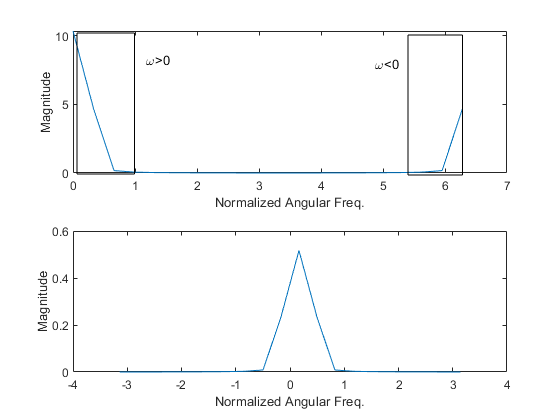
\includegraphics[width=0.45\textwidth]{p521.png}
	\caption{DFT before shifting and after shifting}
	\label{fig:p521.png}
\end{figure}

\subsection{Zero Padding of Input}
The spacing between samples of the DTFT is determined by the number of points in the DFT. This can lead to surprising results when the number of samples is too small. When the number of samples within a sampling interval is less than the Nyquist frequency
\begin{equation}
	N>F_{\text{Nyquist}}=BT_{S}
\end{equation}
, the signal can no longer be recovered due to spectrum overlapping.

A larger sampling frequency increases the sampling frequency, and the frequency domain convolution acts as sinc interpolation that improves the similarity between the digital spectrum and the theoretical analog spectrum.
\begin{equation}
	\mathcal{F} (x[n](u(n)-u(n+L)))=U[e^{j\omega }]*\text{sinc}(\omega L)
\end{equation}
The demonstration Fig.\ref{fig:p522.png} from the following code is evident to this equation. A larger number of samples per interval produces a finer FFT spectrum.

\begin{figure}[htpb]
	\centering
	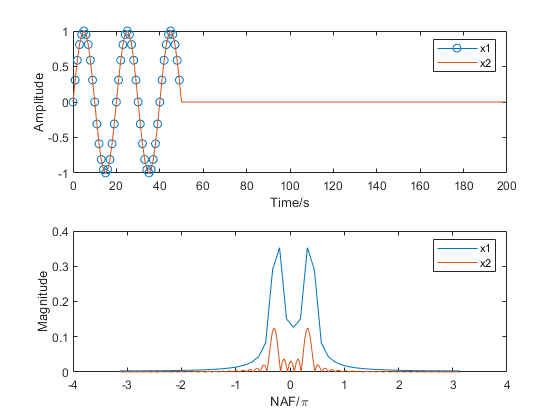
\includegraphics[width=0.45\textwidth]{p522.png}
	\caption{50 samples versus 200 samples}
	\label{fig:p522.png}
\end{figure}

\section{Fast Fourier Transformation}

\subsection{Single Stage Divide-Conquer}
The divide-conquer method of FFT computation are composed by many consequentially stages of divide, conquer and merge. For the final and the largest stage, the steps can be programmed as following MATLAB code:

\begin{lstlisting}[language=matlab,style=matlab]
function X=dc1DFT(x)
    xe=x(1:2:length(x)-1);
    fxe=DFTsum(xe,length(xe));
    xo=x(2:2:length(x));
    fxo=DFTsum(xo,length(xo));
    twi=exp(-1j*2*pi*(0:length(x)/2-1)/length(x));
    X=[(fxe+fxo.*twi),(fxe-fxo.*twi)];
end
\end{lstlisting}

This code is a direct translation of equation (7) where the \lstinline{fxe,fxo} are variable representation of the \( N/2 \)  DFT of even and odd sequence \( X_{0}, X_{1} \).

The number of multiplication can be easily obtained by analyzing the computations involved in the \lstinline{dc1DFT(x)} function. The matrix implementation of DFT executes one real matrix multiplication to build the Vandermonde matrix, and then executes complex matrix multiplications twice to generate the twiddle matrix and apply the DFT transformation.

\begin{lstlisting}[language=matlab, style=matlab]
function Xk=DFTsum(xn,N)
	n=0:N-1;
	nk=n'*n; % n^2 real
	WNnk=exp(-1j*2*pi/N).^nk; % n^2 complex
	Xk=xn*WNnk; % n^2 complex
end
\end{lstlisting}

Therefore, one matrix DFT requires \( n^2 \) real multiplications and \( 2n^2 \) complex multiplications, which accounts as \( 5n^2 \) real multiplications eventually.

The number of multiplications executed in \lstinline{dc1DFT()} can be divided into two parts, one is the butterfly computation and twiddle factor generation that costs \( 2n \) complex multiplications, the other is the two \lstinline{dcDFT()} with size \( n/2 \) and requires \( 5n^{2}/4 \) real multiplications. Merging the two parts together, the \lstinline{dcDFT()} uses \( 4n+5/4\ n^{2} \) real multiplications.

\subsection{Recursive and Iterative Divide-Conquer}

The subroutine \lstinline{DFTsum} invoked by the single-stage divide-conquer FFT program can be substituted by another divide-conquer subroutine, and the only difference between the upper stage and the lower stage of recursion is the size of the input vector. Since the size of input vector can be conveniently controlled by specifying the initial and final indices, the iterative subroutine is reusable and hardware accelerations such as MKL are able to be applied.

The operations that are to be implemented in the reusable \lstinline{dcDFT(x)} includes generation of corresponding twiddle factor \( W_{N}^{k} \) and the in-situ vector update. Both of the two operations are already optimized in many mathematical libraries, and the existing accelerations has been invoked automatically in MATLAB.

Based on the backward inference of the input sequence from the recursive results, it is clear that the initial input sequence needs to be rearranged in reverse binary order, i.e., the indices of the original sequence are converted to binary numbers, and then converted back to decimal after a bit inversion.

\lstinputlisting[language=matlab,style=matlab]{FFT1.m}

The Rader approach of bit inversion is of \( \mathcal{O} (\log n) \) time complexity, exponentially faster than naively for loop:

\lstinputlisting[language=matlab,style=matlab]{Reverse_Rader.m}

\end{document}